\documentclass[12pt,a4paper]{article}
\usepackage[utf8]{inputenc}
\usepackage[russian]{babel}
\usepackage[width=17cm,top=1cm,height=27cm]{geometry}
\usepackage{graphicx}
\title{Численные методы(Мусаева)}

\date{May 2019}

\begin{document}
\begin{titlepage}
\begin{center}
2019 год
\vspace {8cm}



{ \LARGEПрактикум по численным методам:\\ методы решения систем уравнений }\\
\vspace {8cm}
\bigskip Мусаева Аида, группа 208
\end{center}
\vfill


\vfill

\end{titlepage}
\section{Решение краевой задачи для линейного дифференциального уравнения второго порядка методом прогонки}
\text{
Пусть на отрезке $[a,b]$ требуется найти решение диффурунциального уравнения\\
$y''+p(x)y'+q(x)y=f(x)$,\\
удовлетворяюшее следующим краевым условиям:\\
$c_1y(a)+c_2y'(a)=c,d_1y(b)+d_2y'(b)=d \\
|c_1|+|c_2| \ne 0, |d_1|+|d_2| \ne 0$\\\\
Сначало необходимо вычислить:\\
$\beta_0=c_1h-c_2, \gamma_0=c_2, \phi_0=hc\\ \phi_i=f(x_i)h^2, \alpha_i=1-\frac{1}{2}p(x_i)h,\beta_i=q_ih^2-2, \gamma_i=1+\frac{1}{2}p(x_i)h, i=1,...,n-1\\
\alpha_n=-d_2, \beta_n=hd_1+d_2, \phi_n=hd$\\\\
Решение ищем в виде:
$y_i=u_1+v_iy_{i+1}$\\
Где $u_1= \frac{\phi_i - \alpha_iu_{i-1}}{\beta_i+\alpha_iv_i},
Где v_1= -\frac{\gamma_i}{\beta_i+\alpha_iv_{i-1}} $\\\\
Задание:\\
$ y''+sh(x)y'+ch(x)y=\frac{1}{1+x^2}\\
0.5y(0)+0.3y'(0)=0,0.16y(1)+0.64y'(1)=0.3$
}
\subsection{Код программы}
\begin{verbatim}
import numpy as np
import matplotlib.pyplot as plt

def p(x):
    return np.sinh(x)
def q(x):
    return np.cosh(x)
def f(x):
    return 1 / (1 + x ** 2)


def tridiagMat(p, q, f, a, b, c1, c2, c, d1, d2, d, n):
    h = (b - a) / n
    u = np.zeros(n + 1)
    v = np.zeros(n + 1)
    x = np.zeros(n + 1)
    y = np.zeros(n + 1)
    alp = np.zeros(n + 1)
    bet = np.zeros(n + 1)
    gam = np.zeros(n + 1)
    phi = np.zeros(n + 1)

    x[0] = a
    i = 1
    u[0] = c * h / (c1 * h - c2)
    v[0] = -c2 / (c1 * h - c2)

    while True:
        x[i] = x[i - 1] + h
        alp[i] = 1 - p(x[i]) * h / 2
        bet[i] = h ** 2 * q(x[i]) - 2
        gam[i] = 1 + p(x[i]) * h / 2
        phi[i] = (h ** 2) * f(x[i])
        v[i] = -gam[i] / (bet[i] + alp[i] * v[i - 1])
        u[i] = (phi[i] - alp[i] * u[i - 1]) / (bet[i] + alp[i] * v[i])
        if i == n - 1:
            break
        i += 1
    x[n] = b
    alp[n] = -d2
    bet[n] = h * d1 + d2
    phi[n] = h * d
    v[n] = 0
    u[n] = (phi[n] - alp[n] * u[n - 1]) / bet[n]
    y[n] = u[n]
    i = n - 1
    while True:
        y[i] = u[i] + y[i + 1] * v[i]
        if i == 0:
            break
        i -= 1
    return {'x': x, 'y': y}
a = 0
b = 1
c1 = 0.5
c2 = 0.3
c = 0
d1 = 0.16
d2 = 0.64
d = 0.3
n = 700


ans = tridiagMat(p, q, f, a, b, c1, c2, c, d1, d2, d, n)
plt.plot(ans['x'], ans['y'])
plt.show()
\end{verbatim}
\vspace {8cm}
\subsection{Результат работы программы}

\begin{figure}[h]
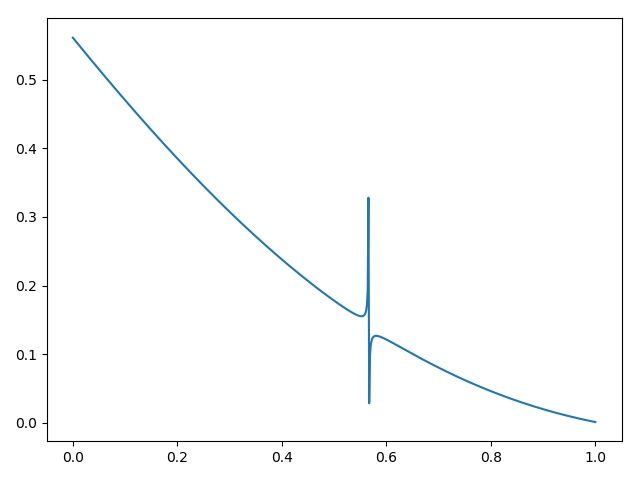
\includegraphics[width=\linewidth]{pic.jpg}
\caption{}
\label{fig:}
\end{figure}

\section{Решение нелинейной системы методом простых итераций}
\text{Осуществляется аналогично методу простых итераций для одного уравнения\\
Задание:\\
}\begin{displaymath}
\left\{ \begin{array}{ll}
\cos(x_1+0.5)-x_2=2 \\
x_2-\cos(x_1)=3

\end{array} \right.
\end{displaymath}
\subsection{Код программы}
\begin{verbatim}
import numpy as np
def f(x):
    return np.array([np.sin(x[1])/2-1/2, np.cos(x[0]+0.5)-2])

def Iterative(f, x0, eps=1e-6):
    k = 0
    while True:
        x = f(x0)
        if (np.linalg.norm(x - x0) < eps):
            return x0, k
        x0 = x
        k += 1
x0 = np.array([0, 0])
print(Iterative(f, x0))
\end{verbatim}
\subsection{Результат работы программы}
\text{
\begin{displaymath}
\mathbf{X} =
\left( \begin{array}{c}
-0.94501095 \\
-1.09739416 \\
\end{array} \right)
\end{displaymath}
13 итераций
}

\end{document}
